% Chapter Template

\chapter{Requirements and Analysis} % Main chapter title

\label{Chapter4} % Change X to a consecutive number; for referencing this chapter elsewhere, use \ref{ChapterX}

\lhead{Chapter 4. \emph{Requirements and Analysis}} % Change X to a consecutive number; this is for the header on each page - perhaps a shortened title

%------------------------------------------------------------------
%	SECTION 1
%------------------------------------------------------------------

\section{Requirements}
Application requirements describe a particular design of this project. The requirements include functional requirements and non-functional requirements.

%-----------------------------------
%	SUBSECTION 1
%-----------------------------------
\subsection{Functional Requirements}

Functional requirements consist of user requirement and system requirement. This is the information that explains the all the functions performed by user and system. 
For this application the user and the system can perform the following functions:\\
\textbf{User:}\\
- Can use images from gallery to counting.\\
- Can use images taken by iPhone camera to counting.\\
- Can see the result of number sheets of cloth.\\
\textbf{System:}\\
- Can count sheets of cloth that it is placed overlay with acceptable accuracy.


%-----------------------------------
%	SUBSECTION 2
%-----------------------------------

\subsection{Non-Functional Requirements}
Non-functional requirements include user requirement and system requirement. This is the requirements that emphasize on the scope of work of the application. 
For this application the user and the system can perform the following functions:\\
- The system can count sheets of cloth faster than manual counting.\\
- User interface of application is simple and easy to use.\\
- The system can be developed further features.\\
%------------------------------------------------------------------
%	SECTION 2
%------------------------------------------------------------------
\section{Use Case}
A use case is a list of steps defining in Unified Modeling Language (UML). It consists of use case diagram and use case description.
%------------------------------------------------------------------
%	SUBSECTION 2-1
%------------------------------------------------------------------

\subsection{Use Case Diagram}
Use case diagram is a representation of a user's interaction with the system and depicting the specifications of a use case. It can portray the different types of users of a system and the various ways that they interact with the system as shown in Figure \ref{fig:f401}.
\begin{figure}[t]
	\centering
	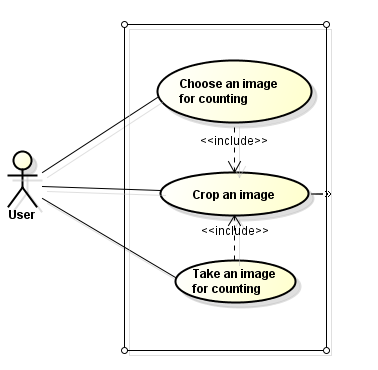
\includegraphics[scale=1]{f401.png}
	\caption{System’s Use Case Diagram}
	\label{fig:f401}
\end{figure}

Users can interact with the application in three different tasks. First, user can choose an image from gallery to counting. Second, users can take an image from camera application to counting. Both tasks are input of application. Final task user can crop an image with particular area in an image to receiving the acceptable result. Note that, the users have to start from the application's input tasks.
%------------------------------------------------------------------
%	SUBSECTION 2-2
%------------------------------------------------------------------
\subsection{Use Case Description}
Use case description describes user and system both are interaction in details. The details of all tasks are explained in tables \ref{tab:t401} - \ref{tab:t403}. 

Table \ref{tab:t401} describes about the task of choosing an image.  This task allows the user to choose an image from the image gallery. The step of the tasks can be shown as in the following. First, the user presses a gallery button. The system responds by showing the screen of image gallery. Then the user chooses an image. The image will be shown on the screen. In case of alternative flow, user dose not choose the image from gallery, the system will display a message. Then user gets an image from photography.

Table \ref{tab:t402} describes about the task of taking an image. This task allows the user to photograph the piled of sheets of cloth. The step of the tasks can be shown as in the following. First, the user presses the camera button. The iPhone’s camera is opened. Then the user takes an image. The image is shown on the iPhone’s screen. In case of alternative flow, user does not photograph, the system will display a message. Then the user chooses an image from gallery. 

Table \ref{tab:t403} describes about the task of cropping an image. This task allows the user to crop an image that is shown on iPhone’s screen. The step of the tasks can be shown as in the following. First, user crops the desired area of the image. Then presses use image button. The cropped image and the message of counting result are shown on the screen of iPhone.\\
\begin{table}[t]
	\begin{center}	
	\begin{tabular}[t]{|l|p{5cm} |p{5cm}|}
		\hline
		Use case & \multicolumn{2}{l}{Choose an image from gallery for counting} \vline\\
		\hline
		Actor &\multicolumn{2}{l} {User}\vline\\
		\hline
		Pre-condition & \multicolumn{2}{l}{The image stored in image galley on the iPhone.}\vline\\
		\hline
		Post-condition & \multicolumn{2}{l}{The image is shown on the screen of the iPhone.}\vline\\
		\hline
		Flow of event & Actor input & System response\\
		& 1) User presses the gallery button. & \\ 
		&& 2) The iPhone's screen shows the image gallery.\\
		& 3) User chooses an image from the gallery. & \\
		&& 4) The image is shown on the screen of iPhone.\\
		\hline
		Alternative flow & 1) User does not press the gallery button. &\\
		&& 2) System display message "Please choose an image"\\
		& 3) User gets an image from photography. &\\
		\hline
	\end{tabular}
	\caption{Use case diagram of choosing an image}
	\label{tab:t401}
\end{center}
\end{table}

\begin{table}[t]
	\begin{center}
		\begin{tabular}{|l|p{5cm} |p{5cm}|}
			\hline
			Use case & \multicolumn{2}{l}{Take an image for counting} \vline\\
			\hline
			Actor &\multicolumn{2}{l} {User}\vline\\
			\hline
			Pre-condition & \multicolumn{2}{l}{The image does not store in image gallery on the iPhone.}\vline\\
			\hline
			Post-condition & \multicolumn{2}{l}{The image is shown on the screen of the iPhone.}\vline\\
			\hline
			Flow of event & Actor input & System response\\
			& 1) User presses the camera button. & \\ 
			&& 2) The iPhone's camera is opened.\\
			& 3) User photographs an image. & \\
			&& 4) The image is shown on the screen of iPhone.\\
			\hline
			Alternative flow & 1) User does not press the camera button. &\\
			&& 2) System display message "Please choose an image"\\
			& 3) User chooses an image from gallery. &\\
			\hline
		\end{tabular}
		\caption{Use case diagram of taking an image}
		\label{tab:t402}
	\end{center}
\end{table}
\begin{table}[t]
	\begin{center}
		\begin{tabular}{|l|p{5cm} |p{5cm}|}
			\hline
			Use case & \multicolumn{2}{l}{Crop an image} \vline\\
			\hline
			Actor &\multicolumn{2}{l} {User}\vline\\
			\hline
			Pre-condition & \multicolumn{2}{l}{The image does not store in image gallery on the iPhone.}\vline\\
			\hline
			Post-condition & \multicolumn{2}{l}{The image is shown on the screen of the iPhone.}\vline\\
			\hline
			Flow of event & Actor input & System response\\
			& 1) User crops the desired area on image. & \\ 
			& 2) User presses use button.& \\
			&& 3) The system cropped and shows the cropped image.  \\
			&& 4) The message of counting result is shown on the screen of iPhone.\\
			\hline
		\end{tabular}
		\caption{Use case diagram of cropping an image}
		\label{tab:t403}
	\end{center}
\end{table}
%------------------------------------------------------------------
%	SUBSECTION 2-3
%------------------------------------------------------------------

\section{Activity Diagram}
Activity diagram are a graphical that represents a work-flow of stepwise activities and actions with support for concurrency.
\begin{figure}[t]
	\centering
	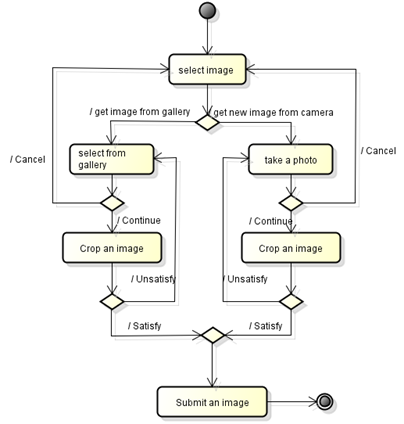
\includegraphics[scale=1]{f402.png}
	\caption{Activity diagram of application}
	\label{fig:f402}
\end{figure}

Figure \ref{fig:f402} describes flows of the application. Starting from a black circle at the top of the diagram, a user can select one of the two possible ways in order to obtain an input image: a) get an image from the gallery or b) get a new image from photographing. Then the user has to crop the image. The result will be an image with only the stack of cloths without background. Note that before the step of submitting the image, the user can cancel the task. This action will take the user back to the previous step.

This chapter presents all of requirements, use case diagram and activity diagram. It will be applied for software design in next chapter.
